%% SECTION HEADER /////////////////////////////////////////////////////////////////////////////////////
\section{Experimental Setup Configuration}
\label{sec:setup}

%% SECTION CONTENT ////////////////////////////////////////////////////////////////////////////////////

The presented model was validated with results from two experimental studies.
The first one was performed for determination of the full wavefield of the propagating waves by the \ac{sldv} (Polytec PSV–400).
The second study was performed for wave acquisition by the \ac{pzt} sensor.
The schematic of the experimental setup is shown in Figure~\ref{fig:setup}.
The sample of interest was a not-regular hexagonal aluminium honeycomb bonded to one \ac{cfrp} plate  using the epoxy adhesive (Loctite EA3479B) as shown in Figure~\ref{fig:honeycomb}(\textbf{a}).%PF: label acc. to figure caption.
The subject of the parametric study was the effect of the disbond size on the propagating GW.

\begin{figure}[H]
	%	\begin{center}
	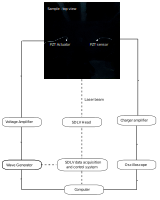
\includegraphics[width=1\linewidth]{Chapter_6/setup}
	%	\end{center}
	\caption{Experimental setup for the (1) \ac{sldv} measurement---dashed line and (2) PZT wave acquisition---solid line.}
	\label{fig:setup}
\end{figure}
\vspace{-12pt}
\begin{figure}[H]
	%	\begin{center}
	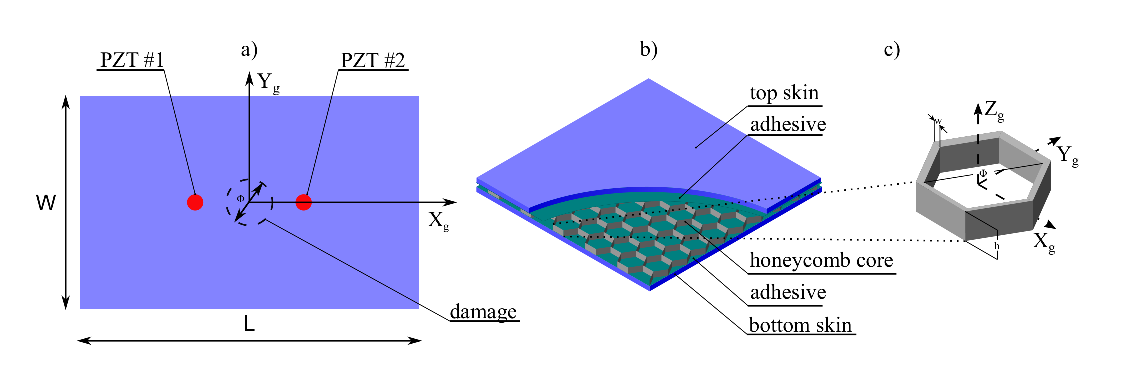
\includegraphics[width=1\linewidth]{Chapter_6/honeycomb}
	%	\end{center}
	\caption{Sample configuration: (\textbf{a}) top view of the sample, (\textbf{b}) honeycomb sandwich substructures and (\textbf{c}) details of the honeycomb cell.}
	\label{fig:honeycomb}
\end{figure}


After a reference measurement was made on an intact sample, several measurements were taken for the subsequent damage introduced on the same specimen.
The circular area of the core was detached from the adhesive at the center of the plate using a sharp hooked tool.
For this purpose, the bottom skin was omitted so that damage could be introduced.
The damage size was controlled by its diameter \(\Phi_D=\left [10, 30, 50, 70, 90, 110, 130 \right ]\) mm.

The generation and reception of elastic waves were achieved with a pair of \ac{pzt} transducers mounted on the skin top surface with the cyanoacrylate glue.
The coordinates of the actuator were \((x_1,y_1)=(-100,0)\) mm,	and for the sensor, \((x_2,y_2)=(100,0)\) mm.
The dimensions of the sample components were as follows:
\begin{itemize}
	\item \ac{cfrp} skin: \(L \times W \times H = 500 \times 500\ \times 1.5\) mm,
	\item Aluminium core: \(g=14.5\) mm, \(w=0.1\) mm, \(h_1=11\) mm, \(h_2=5\) mm, \(l_1=10.4\) mm, \(l_2=6\) mm,
	\item Epoxy adhesive: \(L\times W \times H = 500 \times 500 \times 0.3\) mm,
	\item NCE51 \ac{pzt}: \(\Phi_{PZT}=10\) mm, \(h=0.5\) mm,
	\item Cyanoacrylate glue: \(\Phi_{CG}=10\) mm, \(h=0.05\) mm.
\end{itemize}

The \(N_c=5\) cycle Hann windowed signal at carrier frequencies \mbox{\(f_c=[75,100,125,150]\) kHz} was generated using an arbitrary waveform generator (National Instruments, PXI 5413).
The signal was amplified 40 times and supplied to the \ac{pzt} actuator (Noliac, NCE51).
Each measurement was conducted in the room temperature and averaged 20~times in order to improve the signal to noise ratio.